\documentclass[
reprint,amsmath,amssymb,aps]{revtex4-2}

\usepackage{graphicx}
\usepackage{dcolumn}
\usepackage{bm}
\usepackage{float}
\usepackage{tabularx}
\usepackage{multirow}
\usepackage{braket}
\usepackage{amsmath}


\begin{document}

\preprint{APS/123-QED}

\title{Spin dynamics and magnetic bistability in single Dy adatoms on graphene/Ir(111)
studied by SP-STM}

\author{A. Curcella}
\affiliation{Institute of Physics, Ecole Polytechnique Fédérale de Lausanne, CH-1015 Lausanne, Switzerland}

\author{D. Sblendorio}
\affiliation{Institute of Physics, Ecole Polytechnique Fédérale de Lausanne, CH-1015 Lausanne, Switzerland}

\author{S. Rusponi}
\affiliation{Institute of Physics, Ecole Polytechnique Fédérale de Lausanne, CH-1015 Lausanne, Switzerland}

\author{M. Pivetta}
\affiliation{Institute of Physics, Ecole Polytechnique Fédérale de Lausanne, CH-1015 Lausanne, Switzerland}

\author{F. Patthey}
\affiliation{Institute of Physics, Ecole Polytechnique Fédérale de Lausanne, CH-1015 Lausanne, Switzerland}

\author{H. Brune}
\affiliation{Institute of Physics, Ecole Polytechnique Fédérale de Lausanne, CH-1015 Lausanne, Switzerland}
 

\begin{abstract}
The importance of a comprehensive description of spin dynamics at the atomic-scale is generated by the persistent interest in downscaling electronic devices and the desire for long-living qubits for quantum computing. In this work we investigate the magnetic bistability of single Dy adatoms on graphene/Ir(111) by means of spin-polarized scanning tunneling spectroscopy. We show that the intra-atomic exchange interaction between internal \textit{4f} and external \textit{5d6s} polarized shells modifies the magnetization reversal pathways. This affects the spin-lifetimes of the Dy adatoms, and also changes the effect of spin-pumping induced by tunneling electrons. These evidences offer new insights in the description of spin dynamics of single-atom magnets at surfaces. 
\end{abstract}

\maketitle


%Manipulation of the magnetic states of nano-objects and in surface adsorbed single adatoms offer novel avenues for exploring the fundamental physics that determine their behavior. Understanding this behavior is essential for the development of future spintronic devices and the realization of ultra-high-density magnetic memory [citations...]. The injection of a spin-polarized current can efficiently reorient the magnetization of a nanomagnet \citep{Khajetoorians2013,krause_joule_2011,loth2010}, enabling the possibility of reading and writing of the magnetic states.
%Dysprosium atoms adsorbed on a single graphene layer grown on Ir(111) were identified as stable single-atom magnets \citep{baltic2016}. Previous scanning tunneling microscopy (STM) studies revealed these atoms self assemble into a highly-ordered superlattice after annealing at 40~K \citep{baltic2016,pivetta2018}. Obtaining uniformly dispersed bistable magnetic nanostructures on a decoupling atomic layer is a paramount achievement for the development of ultra-high magnetic memory densities [citations]. Previous x-ray magnetic circular dichroism (XMCD) measurements revealed that Dy adatoms on graphene/Ir(111) possess a \textit{4f$^{\:10}$} occupation, a \textit{J} = 8 total angular momentum identical to Dy in the gas phase, and a \textit{J$_z$} = $\pm$7 out-of-plane magnetic ground state \citep{baltic2016,baltic2018}. The measured spin lifetimes are of the order of 1000~s at 2.5~K.
%However, the lifetimes obtained by XMCD are limited by the interaction of the adatoms with photon-induced secondary electrons. The extrapolation of the intrinsic magnetization lifetime at zero photon flux represents a lower bound estimate.

Coherent spin manipulation and reading/writing the state of stable single-atom magnets represent two of the milestones of modern spintronics research \cite{yangCoherentSpinManipulation2019,Natterer2017}. These achievements pave the way towards the realization of coherent spintronic devices and ultra-high density memories based on atomic-scale objects. The former application requires adatoms with a long coherence time and efficient spin manipulation \cite{baumannElectronParamagneticResonance2015,yangCoherentSpinManipulation2019}, while the latter relies on adatoms showing magnetic remanence \cite{baltic2018,donatiMagneticRemanenceSingle2016,Natterer2018} or, as well, bistability in the orbital population \cite{kiralyOrbitallyDerivedSingleatom2018}. The interaction with the environment and the probing method greatly influence these properties in magnetic adatoms \cite{malavolti_MinimallyInvasiveSpin_2020,verlhacAtomicscaleSpinSensing2019a}. A comprehensive record of such interactions can show new ways of tailoring the properties of single-atom magnets, making them suitable for a wide range of applications \cite{kiraly_AtomicBoltzmannMachine_2021,khajetooriansRealizingAllSpinBased2011}.

In the present work, we demonstrate how intra-atomic exchange interaction affects the spin dynamics of isolated Dy atoms adsorbed on a single graphene (gr) layer grown on Ir(111). Dy/gr/Ir(111) is one of the few examples of single atom magnets \cite{Natterer2018,kiralyOrbitallyDerivedSingleatom2018}, and it possesses a spin lifetimes of the order of 1000~s at 2.5~K \cite{baltic2016}. Despite lacking the thermal stability reported for Ho/MgO/Ag(100), this system has other unique properties. Firstly, Dy adatoms self-assemble on the Moiré pattern of gr/Ir(111) after annealing at 40 K \cite{pivettaDirectCaptureElectrostatic2018}. Secondly, it shows an unrivaled magneto-resistive contrast in spin-polarized scanning tunneling microscopy (SP-STM) measurements \cite{pivettaMeasuringIntraAtomicExchange2020}. One can thus obtain an ordered bidimensional array of atomic bits, characterized by a low bit error rate.
However, the spin dynamics governing the bistability of the magnetization in the Dy adatoms still lacks a quantitative  description.
In the following, we present the results of SP-STM  measurements conducted  on  well-isolated  Dy  adatoms on gr/Ir(111). We implement a revised spin model which accounts for the  recently  observed  intra-atomic  interaction  between internal \textit{4f} and  external \textit{5d6s} polarized  shells  \cite{pivettaMeasuringIntraAtomicExchange2020} and compare it to the simplistic case in which this effect is neglected. The revised model offers an improved description for the spin dynamics of rare-earth based single-adatom magnets.

The Dy adatoms adsorb onto the 6-fold symmetrical ($C_{6v}$) graphene hollow site \cite{baltic2018}. The crystal field (eq.~\ref{eqSI:H_CF}) lifts the degeneracy of the magnetic states and gives rise to a strong out-of-plane easy-axis anisotropy.

In a simplified description, the external shells are not polarized, \textit{i.e.} there is no intra-atomic exchange acting in the system (4f model).
%When the intra-atomic exchange is neglected (\textit{i.e.} non-polarized external shells),
The magnetic states $\ket{M}$ are defined solely by the total angular momentum of the \textit{4f} shell $J_{4f}=8$, and its out-of plane component can label these states $\ket{M}=\ket{J^{z}_{4f}}$ (Fig.~\ref{fig:intra}a). The resulting zero-field level scheme is shown in Fig.~\ref{fig:intra}b. The $B_6^6$ term in the crystal field Hamiltonian  $\mathcal{H}_{CF}$ (eq.~\ref{eqSI:H_CF}) mixes the states with $\Delta J^{z}_{4f}=6n$, with $n\in \mathbb{Z}$. The states $\ket{J^{z}_{4f}}=\ket{\pm 6}$ are therefore mixed, with a splitting of $\hbar\omega=1.3 \times 10^{-2}$ meV. The mixing of these states permits the only efficient channel for magnetization reversal, via quantum tunneling of magnetization (QTM) \citep{baltic2016}. The other states lie too high in energy ($E>20$ meV) to participate in the spin dynamics of the Dy adatoms, at our experimental conditions (see Methods).

\begin{figure*}[ht!]
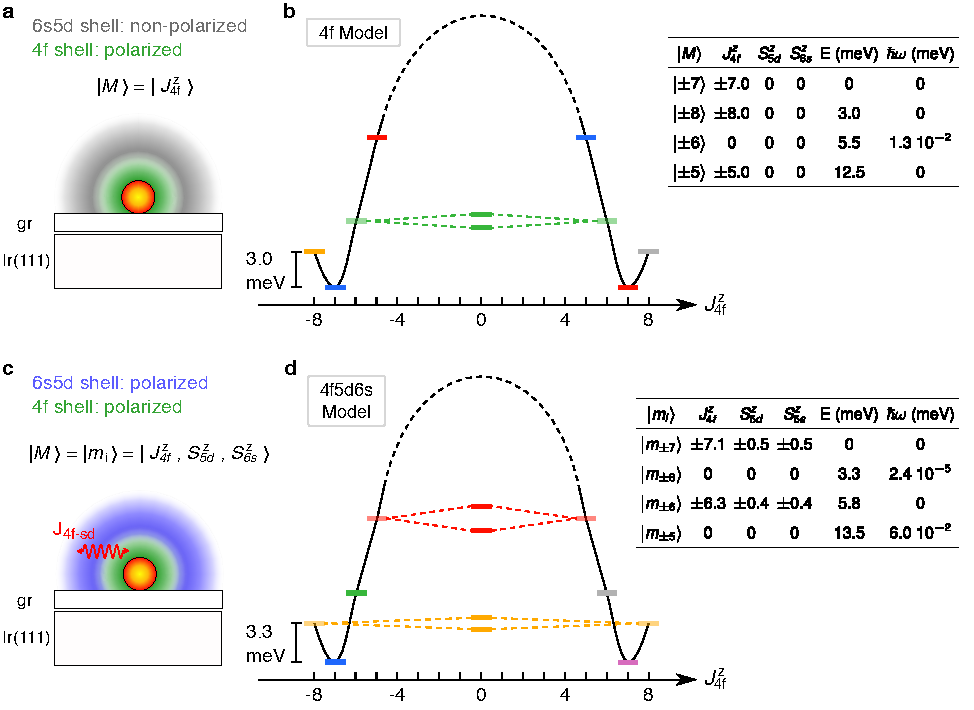
\includegraphics[width=0.98\textwidth]{Fig1_new.pdf}
\caption{\textbf{Comparison between the 4f and 4f5d6s models.} \textbf{a}, Choice of the basis and sketch of the system for the model that considered an unpolarized \textit{5d6s} shell (4f model). \textbf{b}, Corresponding level scheme for the description in (\textbf{a}). States with the same color are mixed by the crystal field. The green dotted line represent the mixing and energy splitting (exaggerated for clarity) of $\ket{\pm6}$ states. Higher energy states are not relevant in the present work, because too high in energy.  The table reports the values of the out-of-plane magnetic moment projection for internal ($J_{4f}^z$) and external ($S^z_{5d}$, $S^z_{6s}$)  electronic shells, energy ($E$) and energy splitting ($\hbar\omega$) for the states $\ket{M}$ depicted in the level scheme. \textbf{c},\textbf{d}, Same as in \textbf{a} and \textbf{b} for the model considering a polarized external shell (4f5d6s model). J$_{4f-sd}$ represents the intra-atomic exchange coupling between \textit{4f} and \textit{6s5d} shells.
\label{fig:intra} }
\end{figure*}

To give a more realistic description, we now consider polarized external \textit{5d-6s} shells \cite{pivettaMeasuringIntraAtomicExchange2020}, and we include the intra-atomic exchange term $\mathcal{H}_{ex}$ (eq.~\ref{eqSI:H_intra}) between internal and external shells in the spin dynamics description (4f5d6s model). 

%The inclusion of the intra-atomic exchange term in the Hamiltonian (\textit{i.e.} polarized external shells), produces a modified level scheme.
As a consequence, we choose a new basis that, in addition to the total angular moment of the \textit{4f} shell, also accounts for the total angular moment of the external \textit{5d-6s} shell, occupied by one electron \cite{pivettaMeasuringIntraAtomicExchange2020,pivettaMeasuringIntraAtomicExchange2020}. However, the orbital component  $L_{4f}$ of the \textit{5d} shell is partially quenched because of hybridization with graphene $\pi$-bands \cite{donati2014}, and for simplicity we assume $L_{4f}$=0; the \textit{s} shells have vanishing orbital component. Thus, both external shells have only a spin angular moment, such that $J_{6s}=S_{6s}=1/2$ and $J_{5d}=S_{5d}=1/2$. The out-of-plane components of the magnetic moment in each shell label the magnetic states of the Dy adatoms $\ket{M}=\ket{m_i}=\ket{J_{4f}^z,S_{5d}^z,S_{6s}^z}$ (table in Fig.~\ref{fig:intra}d).
The intra-atomic exchange couples the \textit{4f} and the \textit{5d6s} shells ferromagnetically (table in Fig.~\ref{fig:intra}d) \cite{pivettaMeasuringIntraAtomicExchange2020}. 
In this new basis, the $B_6^6$ term of the crystal field mixes the states with $\Delta M_{tot}=\Delta J_{4f}^z + \Delta S_{5d}^z + \Delta S_{6s}^z=6n$, $n\in \mathbb{Z}$. This results in the mixing and splitting of the states $\ket{M}=\ket{m_{\pm 5}}$ and $\ket{M}=\ket{m_{\pm 8}}$ (Fig.~\ref{fig:intra}d)
%which have $\Delta M_{tot}\sim 10+1+1 = 12$ and $\Delta M_{tot}\sim 16 +1+1=18$, respectively.
With respect to the former case, two magnetization reversal pathways via QTM exist in the same energy range considered before: the first between $\ket{m_{5}}$ and $\ket{m_{-5}}$, and the second between $\ket{m_{8}}$ and $\ket{m_{-8}}$. Thus, different behaviours are expected depending on the exact description of the system. 

\begin{figure*}[ht!]
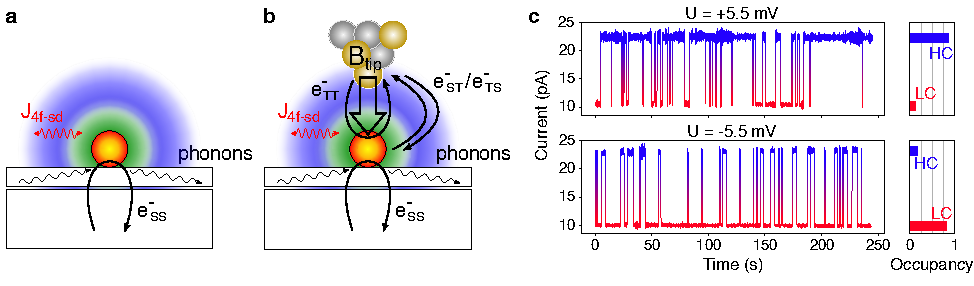
\includegraphics[width=0.98\textwidth]{Fig2_new.pdf}
\caption{\textbf{TS trace and sketch of the scattering processes.} \textbf{a},  Sample TS trace showing a clear asymmetry in occupancy (right graph) between high conductance and and low conductance states ($V_{b} = +5.5$ mV, $T = 6.5$ K). The elastic current $I_{o}$ is the average current measured in each trace and the magnetoresistive component $\pm I_{MR}$ is the absolute difference between $I_{o}$ and $I_{HC}$ or $I_{LC}$, respectively. \textbf{b}, Simplified sketch of the relevant processes considered in the model that influence the measured quantities in tunneling conditions.
\label{fig:no_tip_tip_telegraph} }
\end{figure*}

\begin{figure*}[t!]
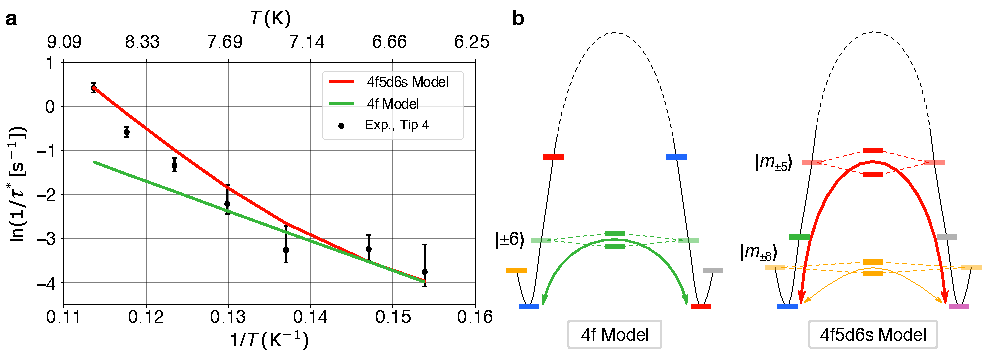
\includegraphics[width=0.99\textwidth]{Fig3_new.pdf}
\caption{\textbf{Variable Temperature Measurements.} \textbf{a}, Arrhenius plot comparing the 4f (red) and 4f5d6s (green) models with the experimental observations (black, $V_b$=1 mV, set current $I$ = 10 pA, in the LC state). The experimental ratio between pure elastic and magnetirestive components is $I_{MR}/I_{o}$ = 0.08±0.01, in good agreement with the calculated  value of $I_{MR}/I_{o}$ = 0.1 (for both models). Error bars in the figure correspond to 95$\%$ confidence intervals calculated using the Agresti-Coull method for binomial distributions for all the data points presented \citep{agresti1998}. \textbf{b}, Level scheme of the two models and corresponding magnetization reversal pathways (arrows). The thickness of the arrows reflects the intensity of the QTM channels.
\label{fig:temp} }
\end{figure*}

SP-STM is the perfect tool to investigate the dynamics of isolated spin \cite{wiesendanger_ObservationVacuumTunneling_1990,Khajetoorians2013,paul_ControlMillisecondSpin_2017,Natterer2017,Natterer2018}. By varying temperature \textit{T}, bias voltage $V_b$ and tunneling current \textit{I}, it is possible to tune the weight of the available relaxation processes (see Fig.~\ref{fig:no_tip_tip_telegraph}), corresponding to selectively switch on the different pathways for reversal; thus, SP-STM allows to discriminate between the two models. 
Fig.~\ref{fig:no_tip_tip_telegraph}a shows an example of constant-height current traces, showing a two-state
telegraph signal (TS). Tunneling current switches between a high conductance (HC) and low conductance (LC) state, corresponding to a parallel and anti-parallel alignment between the majority spin-polarization at the Fermi level of the tip and the magnetization of the adatom, respectively \cite{delgado2010,paul_ControlMillisecondSpin_2017}. From a TS trace we can extract two quantities: the occupancy, defined as the fraction of time that the adatom magnetization is in the high conductance ($\tau_{HC}$) or low conductance ($\tau_{LC}$) state, and the characteristic lifetime $\tau ^*=(\tau_{HC}  \cdot \tau_{LC})/( \tau_{HC} + \tau_{LC})$ \cite{Khajetoorians2013}. 

In Fig.~\ref{fig:temp}a, we show an Arrhenius plot obtained by measuring TS traces on the same Dy adatom for temperatures between 6.5 and 8.8 K. Measurements have been performed at bias $V_b$= 1 mV and set current $I$= 10 pA to minimize the spin-pumping induced by the tip polarization \cite{Khajetoorians2013,paul_ControlMillisecondSpin_2017}. The lifetime $\tau^{*}$ decreases exponentially with increasing temperature, as expected for thermally assisted reversal mechanisms. However, the data points show a kink at around 7.3 K, outlining two different regimes. The one at lower temperature is characterized by a gentle decrease of the spin lifetime with increasing temperature. In the second regime, we observe a much steeper decrease. This observation suggests that two QTM processes are involved in the reversal of the Dy magnetic moment. By increasing the temperature, the relative weight of the transitions shifts in favour of the QTM process associated with higher activation energy (steeper slope).

Fig.~\ref{fig:current} reports the spin lifetimes and occupancy as a function of the tunnelling set current. 

At low bias ($V_d=1$ mV), the tunneling current cannot promote the Dy adatom in the first excited states. Thus, we expect to have only thermally assisted QTM processes. By increasing the current (decreasing tip-adatom distance), the spin-lifetime decreases in agreement with previous observations \cite{paul_ControlMillisecondSpin_2017,Khajetoorians2013,krause_joule_2011}. More interestingly, the occupancy of the HC and LC states appears to be asymmetric (0.6-0.4) at low current and gradually tends to a balanced value (50-50). This means that the process governing the asymmetry in the occupancy at a large tip-sample distance competes against the effect of the tip, that becomes stronger at higher currents, resulting in a net 50-50 occupancy.

Finally, the lifetimes and occupancy as a function of bias, shown in Fig.~\ref{fig:bias}a and b, show a strong spin-torque effect at $\pm$8 mV \cite{Khajetoorians2013,delgadoSpinTransferTorqueSingle2010,balashovInelasticElectronmagnonInteraction2008,krause_joule_2011}: the HC state is favoured at positive bias, while the LC state is preferred at negative bias. The onset in the occupancy, more clearly visible at negative biases between -4 and -6 mV, is accompanied by a fast decrease of the lifetimes, suggesting the activation of a current-induced QTM process.
To reproduce the experimental behaviour, we implement a model using rate equations and a model Hamiltonian containing $\mathcal{H}_{ex}$ and $\mathcal{H}_{CF}$, plus the terms describing the interaction with the substrate and the tip (Fig.~\ref{fig:no_tip_tip_telegraph}b).

\begin{figure}[h!]
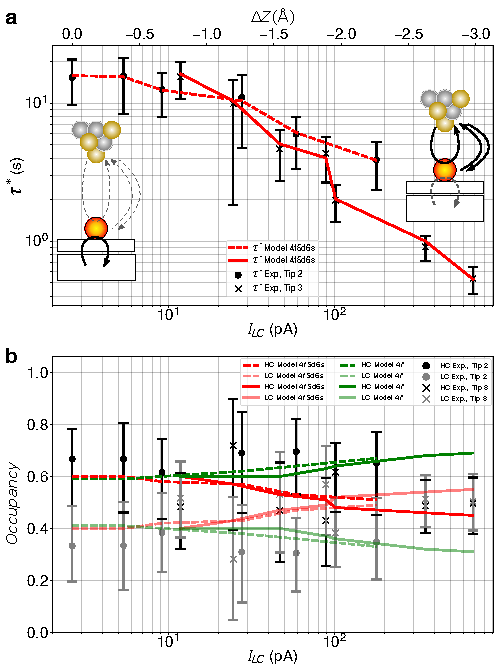
\includegraphics[width=0.5\textwidth]{fig5_final_v3.pdf}
\caption{\textbf{Variable Current Measurements.} \textbf{a}, Lifetime measurements, and \textbf{b}, occupancy as set current (LC state) and corresponding $\Delta Z$ (\AA) distance ($V_{b} = +1$ mV, $T = 6.5$ K). Two datasets are included, indicated with dots (Tip 1) or crosses (Tip 2). $\Delta Z = 0$ is fixed by the lowest current point. The sketches in \textbf{a} show that  at low current the spin dynamics is dominated by $e_{SS}$ scattering, while at higher current $e_{TT}$, $e_{TS}$ and $e_{ST}$ are the dominant contributions. 
\label{fig:current} }
\end{figure}

The intrinsic lifetime of the Dy adatoms is limited by substrate electron and phonon scattering. In addition to these mechanisms, the measured lifetime is determined by further electron scattering channels and the stray magnetic field due to the presence of the STM tip (Fig.~\ref{fig:no_tip_tip_telegraph}b).
To model the coupling between adatom and electron reservoirs (\textit{i.e.} the tip and the substrate), we use a Kondo-type Hamiltonian $\mathcal{H}_{te}$ consistent with previous works \cite{anderson1966,schrieffer1966,appelbaum1967,delgado2010,loth2010,Ternes2015}, which describes four types of electronic exchange interactions: substrate-substrate scattering ($e_{SS}$), tip-tip scattering ($e_{TT}$), and tip-substrate/substrate-tip scattering ($e_{TS}$/$e_{ST}$). In the case of $e_{SS}$ and $e_{TT}$ scattering, the creation or annihilation of an electron hole pair in the electrodes induces a spin transition ($\Delta m=\pm 1$).
Note that, in the case of the 4f model, the spin transition acts directly on the internal \textit{4f} shell, as the external one is not polarized.
Considering the 4f5d6s model, instead, electron scattering induces spin transitions in the external \textit{5d6s} shell. Consequently, the magnetic moment of the $4f$ shell flips due to the intra-atomic exchange coupling between the shells \cite{pivettaMeasuringIntraAtomicExchange2020}.
$e_{SS}$ scattering electrons induce symmetric $\Delta m=\pm 1$ transitions and therefore promote equal occupancy between HC and LC states.
%In the case of tip-tip scattering, the creation or annihilation of an electron hole pair in the tip induces a spin transition ($\Delta m=\pm 1$) in the external \textit{5d6s} shell. 
Differently, the spin-polarized tip is characterized by spin-up $\rho_{T\uparrow}$ and spin-down $\rho_{T\downarrow}$ populations at the Fermi level. The asymmetry in the population implies that $e_{TT}$ scattering induces with a higher probability spin-increasing ($\Delta m=+1$)  or spin-decreasing ($\Delta m=-1$) transitions in the Dy adatom, for $\rho_{T\uparrow}>$0.5 and $\rho_{T\uparrow}<$0.5, respectively.
Note that $e_{SS}$ and $e_{TT}$ electrons affect the spin dynamics of the system, but do not contribute to the tunneling current.
%Note that neither $e_{SS}$ nor $e_{TT}$ electrons contribute to the tunneling current, but they do affect the spin dynamics of the system.

Finally, the electrons that participate in tip-substrate/substrate-tip scattering ($e_{TS}$/$e_{ST}$) define the inelastic component of the current ($I_{in}$). $\mathcal{H}_{te}$ also describes the elastic processes between tunneling electrons and the Dy adatoms, which determine the elastic ($I_0$) and elastic magnetoresistive $I_{MR}$ components of the tunneling current \cite{delgado2010}.
Despite being the only component actively contributing to the spin transitions in the Dy adatoms, $I_{in}$ is orders of magnitude smaller compared to the elastic components. Thus, in the TS traces we approximate the current of the HC state and LC states as $I_0+I_{MR}$ and $I_0-I_{MR}$, as shown in Fig.~\ref{fig:no_tip_tip_telegraph}a.

The transition rates $W_{MM^{\prime}}^{\eta}$ between two states $M,M^{\prime}$ associated with electron scattering from the electrode $\eta=T,S$ (for tip and substrate, respectively) scale with $\zeta^2 \varsigma_{\eta} \varsigma_{\eta^{\prime}}$ (eq.~\ref{eq:elec_rates}), in which $\zeta$ represents the ratio between inelastic and elastic tunneling matrix elements, and
$\varsigma_{\eta}$ quantifies the transmission between the electrode $\eta$ and the adatom.

% The transition rates between two states $M,M^{\prime}$ associated with electron scattering from tip ($e_{TT}$), substrate ($e_{SS}$) and tunneling current ($e_{TS}$/$e_{ST}$) can be expressed as:

% \begin{equation}
%     W_{MM^{\prime}}^{\eta \eta^{\prime}}=\dfrac{2\pi}{\hbar} \zeta^2 \varsigma_{\eta} \varsigma_{\eta^{\prime}} \mathcal{F}_{\eta\eta^{\prime}}( E_{M,M^{\prime}}+V_{\eta \eta^{\prime}} )  w_{MM^{\prime}}^{\eta \eta^{\prime}},
%     \label{eq:elec_rates}
% \end{equation}

% where $\eta,\eta^{\prime}=T,S$. $w_{MM^{\prime}}^{\eta \eta^{\prime}} $ are the tunneling matrix elements squared, $\varsigma_{\eta}$ quantifies the transmission between the electrode $\eta$ and the adatom. $\mathcal{F}_{\eta\eta^{\prime}}$ accounts for the state occupation for a given energy level difference $ E_{M,M^{\prime}}$ and tunnel bias $V_{TS/ST}$.

%For $\eta=\eta^{\prime}$, Eq.~\ref{eq:elec_rates} describes electrons originating and ending in the same electrode ($e_{SS}$, $e_{TT}$), whereas for $\eta \neq \eta^{\prime}$, it describes the scattering from $I_{in}$ ($e_{TS}$, $e_{ST}$). 
We assume $\zeta$ to be independent of the voltage bias $V_b$ and tip-sample distance \cite{fern2009,paul_ControlMillisecondSpin_2017,lorenteEfficientSpinTransitions2009,nussinovNoiseSpectroscopySingle2003}.
$\varsigma_T$ is related to $\varsigma_S$ through the value of the elastic current $I_0$ (eq.~\ref{eq:sigmaT}). The coupling with the substrate $\varsigma_S$ is independent of the tunneling conditions and therefore constant. $\zeta$ and $\varsigma_S$ determine also the value of the magnetoresistive current $I_{MR}$ which scales as $\zeta \varsigma_{T} \varsigma_{S}$.
To account for phonon scattering in the substrate, we implement a two-dimensional phonon bath that can excite and relax the magnetic states of the Dy adatom \cite{cervetti2016,politi_tunneling_1995,Leuenberger2000}. Phonons can be interpreted as a perturbation of the crystal field, and the associated Hamiltonian term $\mathcal{H}_{ph}$ acts only on the internal $4f$-shell. This is true for the 4f model, in which the unpolarized external shell is not affected by a perturbation on the crystal field, but also for the 4f5d6s model, due to the vanishing orbital component of the external \textit{5d6s} shell. We allow transitions with $\Delta m = \pm 1$ and $\Delta m = \pm 2$ \citep{cervetti2016}. 
The transition rates $W_{MM^{\prime}}^{ph}$ between the states $\ket{M}$ and $\ket{M^{\prime}}$ (eq.~\ref{eq:phonon_rates}) depends upon $\nu_{ph}$, which is proportional to the phonon-spin coupling cross section.

% The transition rates between the states $\ket{M}$ and $\ket{M^{\prime}}$ can be expressed as \cite{politi_tunneling_1995, cervetti2016,Leuenberger2000}:

% \begin{equation}
%     \label{eq:phonon_rates}
%     W_{MM^{\prime}}^{ph}=\dfrac{\nu_{ph}}{\rho_{gr} \hbar^3 c^4} \mathcal{P} \left( E_{MM^{\prime}}, T \right) w^{ph}_{MM^{\prime}}
% \end{equation}

% where $\nu_{ph}$ is proportional to the phonon-spin coupling cross section and is equal to $6 \times 10^{-4}$, $c$ is the speed of sound in graphene, $\rho_{gr}$ is the 2D graphene mass density. $\mathcal{P}\left( E_{MM^{\prime}}, T \right)$ depends on the Bose-Einstein distribution at the sample temperature $T$ and the energy difference $E_{MM^{\prime}}$ between states $\ket{M}$ and $\ket{M^{\prime}}$. $w^{ph}_{MM^{\prime}}$ are the phonon matrix elements, acting on the $4f$ shell (see Supplemental).


\begin{figure*}[ht!]
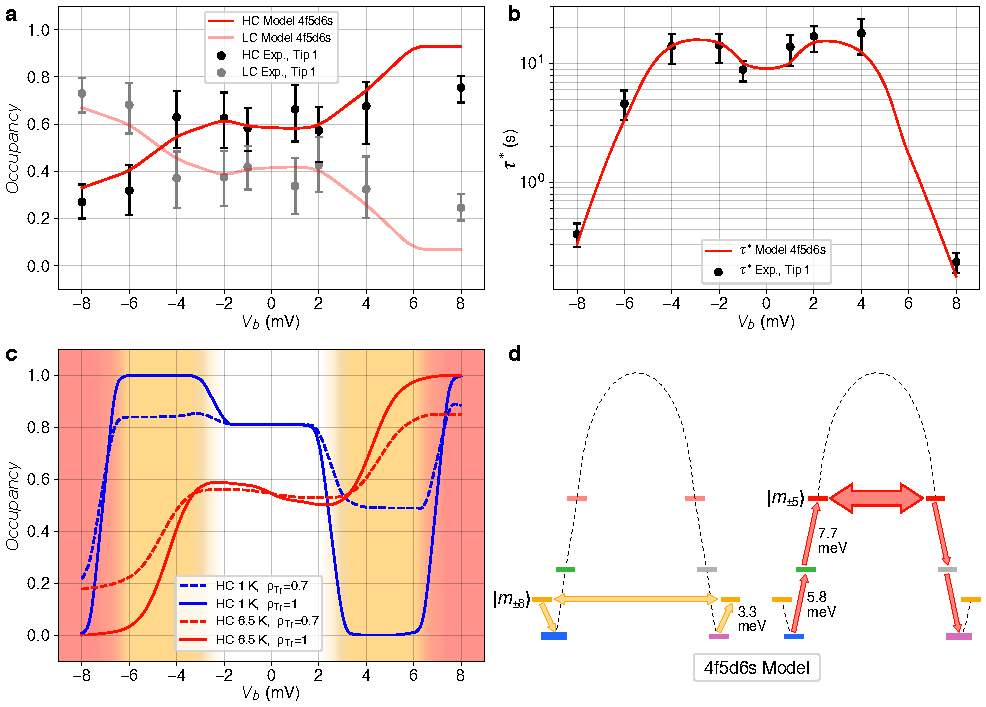
\includegraphics[width=0.99\textwidth]{Fig4_new.pdf}
\caption{\textbf{Variable Bias Measurements.} \textbf{a}, Spin lifetimes, and \textbf{b} occupancy for experimental measurements (black) and model calculations (red) as a function of bias ($T = 6.5$ K, set current I= 10 pA in the LC state). The experimental ratio $I_{MR}/I_{o}$ = 0.18±0.05 while the model value is $I_{MR}/I_{o}$ = 0.11. \textbf{c}, Model calculations of state occupancy as a function of bias at two different temperatures, and tip polarization. White, orange and red backgrounds represents the bias ranges dominated by tip field, $\ket {m_{\pm8}}$ QTM process, $\ket {m_{\pm5}}$ QTM process, respectively. Note that for simplicity, the tip field $B_{tip}$ (100 mT) and $I_o$ (15 pA) is kept constant for each bias, unlike in \textbf{a} and \textbf{b}. \textbf{d}, Level scheme and the dominant reversal pathway for intermediate and high voltage regimes, orange and red in \textbf{c}, respectively. The size of the arrows reflects the strength of the transition. The preferred ground-state is enlarged for clarity.
\label{fig:bias} }
\end{figure*}

A Zeeman term $\mathcal{H}_Z$ (eq.~\ref{eq:zeeman}) in the Hamiltonian describes the influence of the magnetic field produced by the STM tip. The tip field shifts the magnetic states sitting on the opposite sides of the anisotropy barrier, resulting in an energetically preferred ground-state. This manifests experimentally as an asymmetric occupancy of the HC and LC states at low bias ($V_b\sim1$ meV). SP-STM tips can induce both dipolar and exchange-like magnetic interactions between the tip and single adatoms at tunneling distances \cite{yang2019}. The exchange-like component of the field can have a non-trivial dependence on the tip-adatom distance \cite{hauptmannQuantifyingExchangeForces2020,tao_SwitchingSingleSpin_2009,lazoFirstprinciplesStudyMagnetic2011,lazoRoleTipSize2008}. Indeed, the Zeeman term acts only on the polarized shells, \textit{i.e.} only the internal \textit{4f} shell in the 4f model, and on both the internal \textit{4f} and external \textit{5d6s} ones in the 4f5d6s model.

Taking the aforementioned mechanisms into account, we obtain a total Hamiltonian $\mathcal{H}$:

\begin{equation}
\mathcal{H} = \mathcal{H}_{ex} + \mathcal{H}_{Z} + \mathcal{H}_{CF}  + \mathcal{H}_{ph} + \mathcal{H}_{te}
\end{equation}


Note that the intra-atomic exchange $\mathcal{H}_{ex}$ has a vanishing contribution in the case of the simplified 4f model, while it actively couples internal and external shells in the more realistic 4f5d6s model.
By solving the master equation including the transition rates associated with electron scattering $W_{MM^{\prime}}^{\eta}$ and phonon scattering $W_{MM^{\prime}}^{ph}$, we can calculate the occupancy and spin lifetimes $\tau^{*}$ as a function of bias $V_{b}$, temperature $T$, and current $I_{o}$, for the 4f and 4f5d6s models. 
In both cases, we find that the values of $\varsigma_S$=0.064, and  $\nu_{ph}$= $6.0\ 10^{-4}$ give the best agreement with experimental data. Concerning $\zeta$, we obtain a different optimum value in the two descriptions: 0.02 for the 4f model, and 0.3 for the 4f5d6s model. The one order of magnitude difference in the values is justified by the difference between the matrix elements used to calculate the $I_{MR}$ (see eq.~\ref{eq:I_MR}.  Also the values for $B_{tip}$ have been optimized independently in two models (Fig.~\ref{fig:fields}).
The value of $\varsigma_S$ = 0.065 used in our calculations also gives a value of the intrinsic spin-lifetime $\tau_o=962$ s, determined by neglecting tip scattering processes and tip field $B_{tip}$, which is consistent with the extrapolated zero-photon flux XMCD lifetime of 971$\pm$71 seconds at 10 mT and 2.5 K \citep{baltic2016}.

%reproduce the experimental occupancy and characteristic lifetimes measured from TS traces similar to Fig. \ref{fig:no_tip_tip_telegraph}b, as a function of bias $V_{b}$, temperature $T$, and current $I_{o}$. The transition rates defined by Eqs.~\ref{eq:phonon_rates} and~\ref{eq:elec_rates} are used within a master equation to obtain values for $\tau^*$ and state occupancy for a certain set of tunneling conditions \cite{delgado2010,Khajetoorians2013,loth2010,cervetti2016}.

%In Fig.~\ref{fig:temp}a, we show an Arrhenius plot measured on a Dy adatom for temperatures between 6.5 K and 8.8 K. The lifetimes $\tau^*$ decrease exponentially with increasing temperature.
%The slope of the curve in the Arrhenius plot is related to the energy barrier of the transition enabling the magnetization reversal in the Dy adatom. In the same figure, we show the curves determined by each model described in Fig.~\ref{fig:intra}: the model which describes the intra-atomic exchange between the internal \textit{4f} shell and the polarized \textit{5d6s} shell (4f5d6s model) and the model that considers an unpolarized external shell (4f model).
In Fig.~\ref{fig:temp}a, we show the calculated spin-lifetimes as function of temperature for the 4f (green) and the 4f5d6s (red) models. Most notably, the 4f model fails to reproduce the spin lifetime trend at high temperature ($T\sim 8.8$ K). The active pathway for magnetization reversal between $\ket{6}$ and $\ket{-6}$ (see Fig.~\ref{fig:temp}b) lies at 5.5 meV, which corresponds to the slope of the green curve in Fig.~\ref{fig:temp}a. Conversely, the red curve (4f5d6s model) shows a kink at 7.3 K, congruent with the experimental trend. According to our description, temperature-assisted QTM processes between $\ket{m_{-5}}$ and $\ket{m_{5}}$ states become more favored with increasing temperature, while the contribution to magnetic relaxation via $\ket{m_{-8}}$ and $\ket{m_{8}}$ states saturates, because of their low mixing.

Concerning the current dependent measurements in Fig.~\ref{fig:current}, both models can reproduce the spin lifetimes (Fig.~\ref{fig:current}a shows one for clarity), but only the 4f5d6s model can describe the 50-50 occupancy observed at high current. In the low current regime, substrate-substrate electron scattering $e_{SS}$ and the tip field $B_{tip}$ are the dominant mechanisms that determine state occupancy and spin lifetime. The former supports a symmetric occupancy, due to the non-polarized nature of the substrate, while the latter favors the high-conductance state (Fig.~\ref{fig:current}b). As the current is increased, and the tip is moved closer to the Dy adatom, tip-induced scattering plays a larger role and concur with the aforementioned mechanism. Tip electrons favor spin-increasing scattering ($\rho_{T \uparrow} = 0.7$) which drives the magnetization in the $\ket{m_{-7}}$ state (LC state), in opposition to the effect of the tip field. This competition results in an almost symmetric occupation between HC and LC at high currents. Contrarily, the 4f model cannot account for such a behavior, as the magnetization reversal through $\ket{\pm 6}$ states would favor the occupation of the HC state ($\ket{7}$) at high currents, resulting in an asymmetric occupation.


%At positive bias, corresponding to tip-to-substrate tunneling, spin processes parallel to the tip majority spin state at the Fermi level are dominant. If $\rho_{T \uparrow} > 0.5$, this corresponds to spin-increasing, while $\rho_{T \downarrow} > 0.5$ corresponds to spin-decreasing. For $\rho_{T \uparrow} > 0.5 $, the high conductance state corresponds to positive $\ket{m_{+i}}$ states, andthe dominant spin-increasing transitions force the adatom out of the $\ket{m_{7}}$ state into the $\ket{m_{8}}$ excited state. In the 4f5d6s model, QTM from the $\ket{m_{8}}$ state to the $\ket{m_{-8}}$ state results in magnetization reversal. Next, the polarized tunneling electrons facilitate a rapid de-excitation to the $\ket{m_{-7}}$ state. Promotion to the higher energy $\ket{m_{-5}}$ state is less likely, and the adatom is pinned in the $\ket{m_{-7}}$ state, resulting in a preferred low conductance state. Thus, as tip-substrate $e_{TS}$ scattering increases, the occupancy of the low conductance state increases. The experimental points in Fig.~\ref{fig:current}b follow this trend. 

%This trend in occupancy is able to be reproduced only by the 4f5d6s model. The 4f model is characterized by a single reversal pathway through $\ket{\pm 6}$. For $\rho_{T \uparrow} > 0.5 $, the spin-increasing processes that dominate imply that reversal through this pathway from the $\ket{7}$ state is less likely than excitations to the $\ket{8}$ state. Once in the $\ket{8}$ state, the adatom is pinned in the high conductance alignment. For the few reversals that do occur via the pathway $\ket{7} \xrightarrow{} \ket{6} \xrightarrow{} \ket{-6} \xrightarrow{} \ket{-7}$, rapid reversal back to the high conductance state dominates due to the spin-increasing processes. As a result, the 4f model exhibits an increasing asymmetry towards the high conductance state as tip-substrate $e_{TS}$ scattering increases. This trend is not compatible with the experimental measurements. 

%Note that in either model case, if the tip polarization is reversed (\textit{i.e.} $\rho_{T \downarrow} > 0.5$), the high conductance state corresponds instead to the $\ket{m_{-i}}$ states, spin-decreasing processes are dominant at positive bias, and the aforementioned reversal processes remain valid. The sign of the $\ket{m_{\pm i}}$ states is simply reversed. There is no distinguishable difference between the 4f model and 4f5d6s model lifetimes, therefore only the 4f5d6s model is shown in Fig.~\ref{fig:current}a. 
Note that, in order to fit these experimental characteristic lifetimes, a decreasing $B_{tip}$ is needed for both models (see Fig.~\ref{fig:fields}b). It is clear that, while the free parameters used to fit the experimental data allow some flexibility, it is not possible to find a set of parameters within the 4f model that reproduce the slope of the Arrhenius plot and in the high current regime of the variable current occupancy. This emphasizes the importance of including the polarized \textit{5d6s} shell to model the spin dynamics of the Dy system.

The bias dependent measurements (Fig.~\ref{fig:bias}a,b) grant further insights in the in the description offered by the 4f5d6s model. The calculated curves reproduce the spin-torque effect observed in the measurements. The processes that determine the trends in occupancy (Fig.~\ref{fig:bias}a) can be characterized into three regimes. To better elucidate these regimes, and put the variable temperature and current trends into a better context, Fig.~\ref{fig:bias}c displays the 4f5d6s model calculations at $T=1$ K for a fully polarized tip $\rho_{T \uparrow} = 1 $ (blue solid line). For biases between $\pm 2$ meV (white background in Fig.~\ref{fig:bias}c), the occupancy is determined by the tip field $B_{tip}$ which shifts the $\ket{m_{7}}$ state to the lowest energy. Substrate electrons excite the adatom towards the $\ket{m_{\pm8}}$ states in which QTM enables the reversal of the magnetization.

At biases between $+3$ and $+7$ meV (yellow shaded area in Fig.~\ref{fig:bias}c), tunneling electrons can promote transitions towards the first excited states $\ket{m_{\pm 8}}$. For $\rho_{T \uparrow} > 0.5 $, the high conductance state corresponds to the Dy adatom in the $\ket{m_{7}}$ ground state, and tip-to-substrate tunneling is dominated by spin-increasing transitions. The left sketch in Fig.~\ref{fig:bias}d illustrates the reversal pathway allowed at these energies. A completely polarized tip $\rho_{T \uparrow} = 1$ can induce only spin increasing transitions. This forces the adatom out of the $\ket{m_{7}}$ state into the $\ket{m_{8}}$ excited state, in which a QTM process induces the crossing of the magnetic anisotropy barrier towards the $\ket{m_{-8}}$ state. Next, the polarized tunneling electrons promote a rapid de-excitation in the $\ket{m_{-7}}$ state. It is clear that this process pins the adatom in the $\ket{m_{-7}}$ state, corresponding to the low conductance state.

At biases above $+7$ meV (red shaded area in Fig.~\ref{fig:bias}c), transitions between the ground states $\ket{m_{\pm7}}$ and higher excited states $\ket{m_{\pm 6}}$ and $\ket{m_{\pm 5}}$ occur, enabling the magnetization reversal through QTM via $\ket{m_{\pm 5}}$. For $\rho_{T \uparrow} = 1 $, tip-to-substrate tunneling is still completely dominated by spin-increasing transitions, but now the reversal pathway (right sketch in Fig.~\ref{fig:bias}d) forces the Dy adatom into the $\ket{m_{7}}$ state, corresponding to the high conductance state. This process (Fig.~\ref{fig:bias}d, right) dominates over the previous one (Fig.~\ref{fig:bias}d, left) because the QTM channel between $\ket{m_{\pm 5}}$ is $>10^3$ times more efficient than between $\ket{m_{\pm 8}}$. 
The situation is reversed at negative biases, as shown in Fig.~\ref{fig:bias}c: substrate-to-tip tunneling is dominated by spin-decreasing transitions, which force the HC state for $-7<V_d<-3$ meV and LC state for $V_d<-7$ meV. Notice that flipping the polarization of the tip would reverse the occupancy only between $-3<V_d<3$ meV, in which the asymmetry is dominated by the tip field and not by the polarization of tunneling electrons. Partially polarized currents (\textit{e.g.} dashed lines in Fig.~\ref{fig:bias}c) results in a softened spin-torque effect that cannot completely overcome the effect of the tip field, as one can see in the blue dashed curve for $3<V_d<7$ meV in Fig.~\ref{fig:bias}c.  The same foigure also shows how the temperature smears the regimes: the step in the occupancy at high bias ($|V_d|>7$ meV) overcomes the effect of the spin-torque at intermediate bias ($2<|V_d|<7$ meV), which in turn compensates the asymmetry induced by the tip field at low bias ($|V_d|<3$ meV). Thus, the variable temperature measurements presented in Fig.~\ref{fig:temp} explore the effect of increasing this smearing, resulting in an increase in magnetization reversals through the $\ket{m_{\pm 5}}$ states at higher temperatures. On the other hand, the variable current measurements in Fig.~\ref{fig:current} explore the effect of increasing tip-generated scattering processes relative to substrate scattering processes; stressing the importance of the reversal pathways available at low bias and at $T=6.5$ K. Note that as a result of this temperature smearing, we find no appreciable difference between the 4f and 4f5d6s model in fitting the experimental trends as a function of bias (see Fig.~\ref{fig:bias_curr}).

An accurate description of spin dynamics at the atomic scale is essential for the realization of coherent spintronic devices and ultra-high density memories based on atomic-scale objects. The performance of these devices are governed in part by the processes that determine the lifetimes of their magnetic quantum states. The present work ascertains the importance of including the intra-atomic exchange to model these lifetimes and state occupancy. Fundamentally, the inclusion of the intra-atomic exchange does not change the scattering processes and influence of the tip present in the Dy/gr/Ir(111) system. Rather, it modifies the basis and therefore state mixing that determines the available magnetization reversal pathways.

\bibliographystyle{naturemag}
\bibliography{bib.bib}

\end{document}

